\subsection{System design}
% metatext
The \gls{rs} system is designed to consist of multiple parts.
This section contains descriptions of the different parts, and a definition of their responsibilities.

\gls{rs} utilizes the \gls{astep} system which can save locations and route history for users which the \gls{rs} will collect, however the application will need additional data storage to fulfill the set system requirements, therefore, as can be seen on \ref{fig:s2systemdesign}, the application will require a additional database which stores this information.
\begin{figure}[!h]
	\centering
	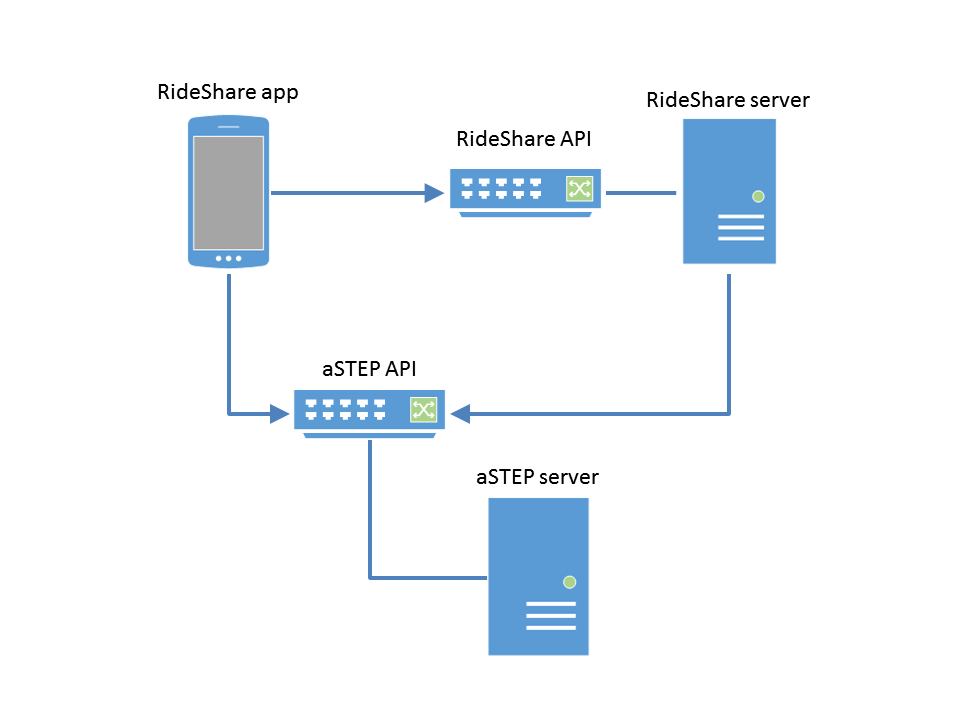
\includegraphics[width=\textwidth]{figures/SystemDesign.png}
	\caption{System design, including all major parts of the solution.}
	\label{fig:s2systemdesign}
\end{figure}
The \gls{rs} server has two main purposes, firstly it should store additional information about the systems users and secondly it should store the score for already calculated scores between given stable routes.
The different purposes and responsibilities of the parts pictured in \ref{fig:s2systemdesign} will be further accounted for in the following text.

% APP RESPONSIBILITY
The \gls{rs} application is responsible for the interaction with the user as well as collecting the location data needed to track routes and recommend ride partners.
The app should communicate with both the \gls{rs} and \gls{astep} server though their respective APIs.

% user management responsibilities
The API and server associated with the \gls{astep} system will be responsible for saving and retrieving location and route data for each user in the system.
The \gls{astep} system is also responsible for the basic user profile, these include an userID and a password.
The user profiles is used to store permissions for which users have access to some given location data.
The \gls{rs} server will be used to store additional info concerning users as well as routes.
For an user we will store additional contact information as well as already calculated ridematching scores for their stable routes. 

This means that an user will both be represented though the \gls{rs} service as well as the \gls{astep} system. 



% Definition of RIDESHARE(TM) server responsibilities
Beyond storing scores for route matches and additional user info the \gls{rs} server will also be responsibly for sending request to the \gls{astep} server, concerning calculations about stable routes and route matches.
